\section{Narzędzia}
\begin{frame}{\insertsection \space-- środowiska programistyczne}
	\begin{columns}
		\column{0.3\textwidth}
			\begin{figure}
				\centering
				
\includegraphics[width=1\linewidth]{../images/DataGrip_icon}
				\label{fig:datagripicon}
			\end{figure}		
		\column{0.3\textwidth}
			\begin{figure}
				\centering
				
\includegraphics[width=1\linewidth]{../images/IntelliJ_IDEA_icon}
				\label{fig:intellijideaicon}
			\end{figure}		
		\column{0.3\textwidth}
			\begin{figure}
				\centering
				
\includegraphics[width=1\linewidth]{../images/WebStorm_icon}
				\label{fig:webstormicon}
			\end{figure}		
	\end{columns}
\end{frame}

\begin{frame}{\insertsection}
		\begin{columns}
		\column{0.5\textwidth}
		\begin{figure}
			\centering
			\label{fig:dockerlogo}
			
\includegraphics[height=1cm,keepaspectratio]{../images/DockerLogo}
		\end{figure}
		\begin{figure}
			\centering
			
\includegraphics[height=1cm,keepaspectratio]{../images/GitLogo}
			\label{fig:gitlogo}
					\begin{figure}
				\centering
				\label{fig:junitlogo}
				
\includegraphics[height=1cm,keepaspectratio]{../images/JUnitLogo}
			\end{figure}
			\begin{figure}
				\centering
				
\includegraphics[height=1cm,keepaspectratio]{../images/PostmanLogo}
				\label{fig:postmanlogo}
			\end{figure}
			\begin{figure}
				\centering
				
\includegraphics[height=1cm,keepaspectratio]{../images/ViteLogo}
				\label{fig:vitelogo}
			\end{figure}
		\end{figure}
		\column{0.5\textwidth}
		\only<1>{\begin{block}{Docker}
			Narzędzie do konteneryzacji.
			\begin{figure}
				\centering
				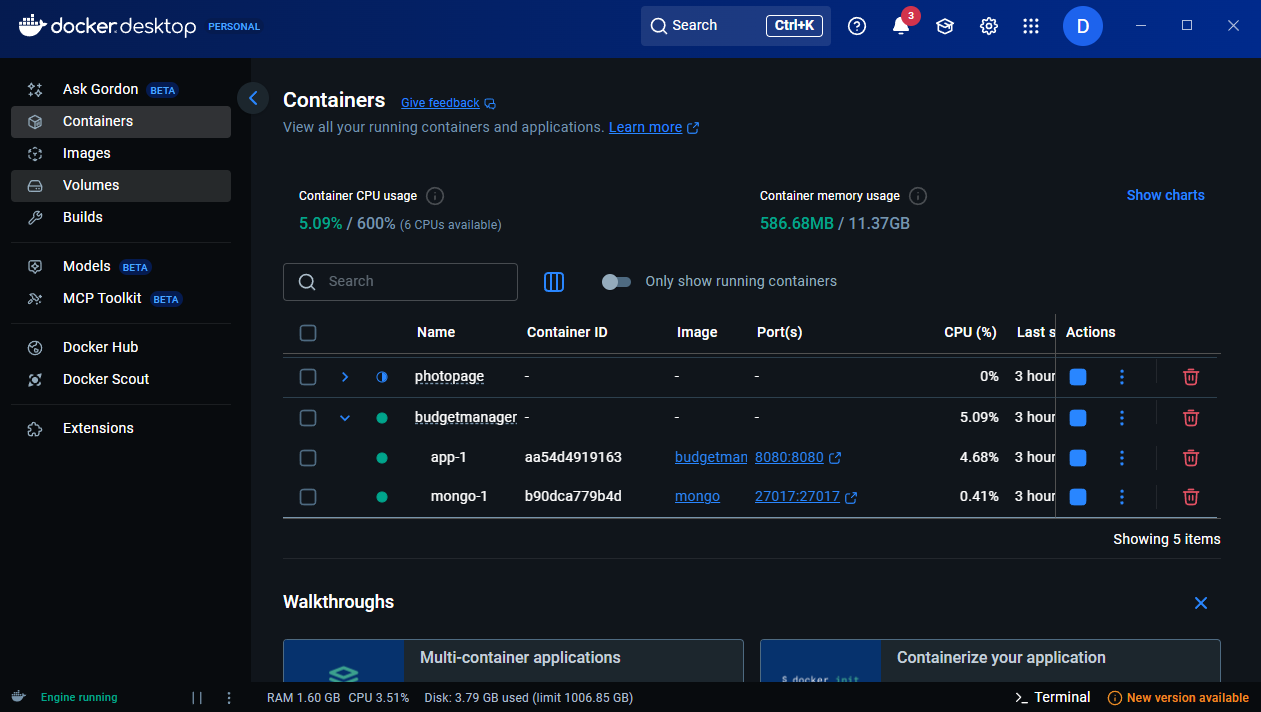
\includegraphics[width=1\linewidth]{../images/DockerApp}
				\label{fig:dockerapp}
			\end{figure}
		\end{block}
		}
		\only<2>{\begin{block}{Kontrola wersji}
			Repozytoria z możliwością zapisywania zmian w kodzie.
		\begin{figure}
			\centering
		
			\label{fig:gitlogs}
			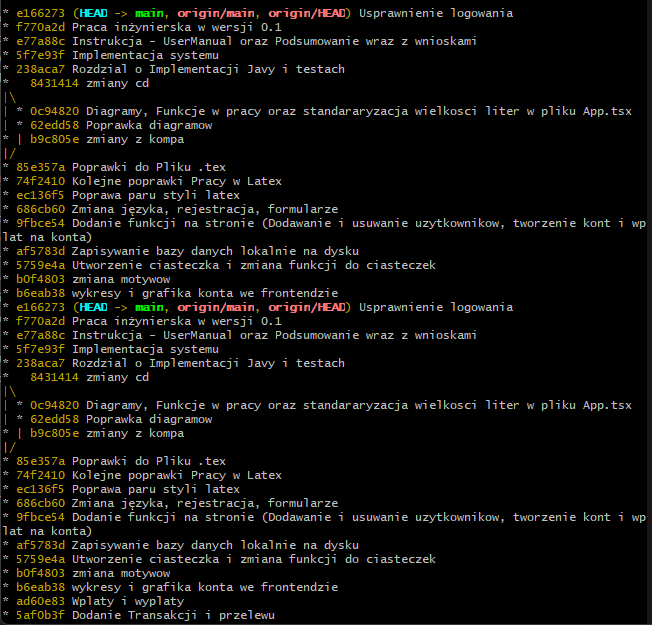
\includegraphics[width=1\linewidth]{../images/GitLogs}
		\end{figure}
		\end{block}
		}
		\only<3>{
		\begin{block}{Testy funkcjonalne}
		Sprawdzanie działania funkcji
		\begin{figure}
			\centering
			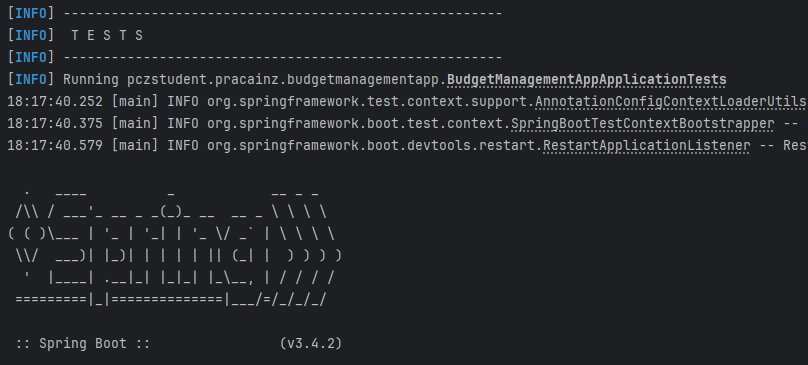
\includegraphics[width=1\linewidth]{../images/Testy}
		
			\label{fig:testy}
		\end{figure}
		\end{block}
		}
		\only<4>{
		\begin{block}{Testy komunikacji}
			Sprawdzanie odpowiedzi na żądania klienta.
		\begin{figure}
			\centering
			\label{fig:postmantest}
			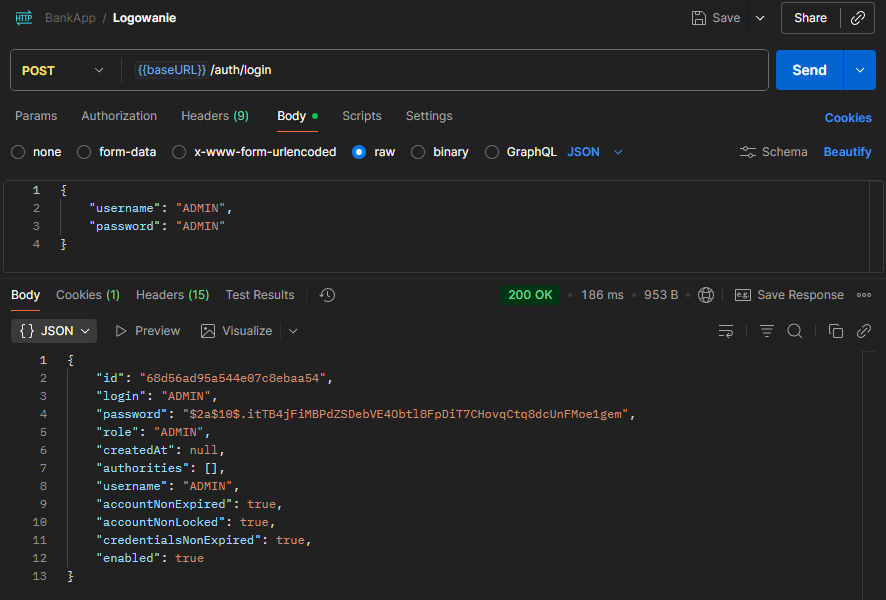
\includegraphics[width=1\linewidth]{../images/PostmanTest}
		\end{figure}
		\end{block}
		}
	\end{columns}
\end{frame}